\documentclass[tikz]{standalone}
\usepackage{pgfplots}
\pgfplotsset{compat=1.15}
\usepackage{mathrsfs}
\usetikzlibrary{arrows,calc}
\usepackage{tkz-euclide}

\pagestyle{empty}

\definecolor{AngleClr}{rgb}{0,0.39215686274509803,0}
\definecolor{ShapeClr}{rgb}{0.6,0.2,0}
\definecolor{BlueClr}{RGB}{5,81,163}

\begin{document}

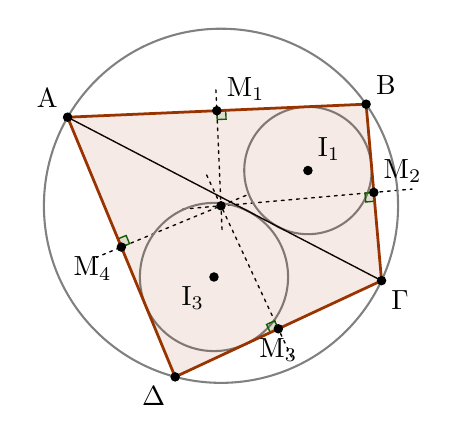
\begin{tikzpicture}[scale=.75]
\tkzSetUpLine[line width=1pt,color=black]
\tkzSetUpPoint[fill=black]

\tkzDefPoint(150:3){A}
\tkzDefPoint(35:3){B}
\tkzDefPoint(-25:3){C}
\tkzDefPoint(-105:3){D}

\tkzDefMidPoint(A,B) \tkzGetPoint{M1}
\tkzDefMidPoint(B,C) \tkzGetPoint{M2}
\tkzDefMidPoint(C,D) \tkzGetPoint{M3}
\tkzDefMidPoint(D,A) \tkzGetPoint{M4}

\tkzDefTriangleCenter[circum](A,B,C) \tkzGetPoint{O}

\tkzDrawSegments[line width=0.5pt,color=black,dashed,dash pattern=on 1pt off 1.75pt,add=0.25 and 0.25](O,M1 O,M2 O,M3 O,M4)

\tkzDefCircle[in](A,B,C) \tkzGetPoints{I1}{i1}
\tkzDrawCircle[line width=0.75](I1,i1)
\tkzDefCircle[in](C,D,A) \tkzGetPoints{I3}{i3}
\tkzDrawCircle[line width=0.75](I3,i3)

\tkzMarkRightAngles[line width=0.5pt, size=.15,color=AngleClr,fill=AngleClr,fill opacity=0.1](O,M1,B O,M2,C O,M3,D O,M4,A)

\tkzDrawCircle[line width=0.75](O,A)

\tkzDrawSegments[line width=0.5pt,color=black](A,C)

\tkzFillPolygon[fill=ShapeClr,fill opacity=0.1](A,B,C,D)
\tkzDrawPolygon[color=ShapeClr](A,B,C,D)


\tkzDrawPoints[size=3](A,B,C,D,I1,I3,M1,M2,M3,M4,O)
\tkzLabelPoint[above left](A){$\rm A$}
\tkzLabelPoint[above right](B){$\rm B$}
\tkzLabelPoint[below right](C){$\rm \Gamma$}
\tkzLabelPoint[below left](D){$\rm \Delta$}

\tkzLabelPoint[above right](I1){$\rm I_1$}
\tkzLabelPoint[below left](I3){$\rm I_3$}

\tkzLabelPoint[above right](M1){$\rm M_1$}
\tkzLabelPoint[above right](M2){$\rm M_2$}
\tkzLabelPoint[below](M3){$\rm M_3$}
\tkzLabelPoint[below left](M4){$\rm M_4$}

\end{tikzpicture}

\end{document}
